
\begin{savequote}[50mm]
Never any knowledge was delivered in the same order it was invented.
%\footnotemark[1]
\qauthor{Sir Francis Bacon}
\end{savequote}

\chapter{Background}
\label{cha:Background}

%\footnotetext[1]{In \textit{Valerius Terminus: Of the Interpretation of Nature}, c. 1603.}
%\setcounter{footnote}{1}

We present the mathematical models we will be considering and the numerical methods we will be using. 

First, we present a general scalar conservation law and the Euler equations. The multiphase flow model will be presented in \cref{cha:MPM}. The properties of the solution to the scalar conservation law are presented in more detail, with a focus on the uniqueness of the solution and entropy conditions.

We then present the numerical methods we will use. We begin with the standard methods for scalar conservation laws and consider their numerical viscosity and flux-difference splitting forms. Convergence and entropy stability of the numerical methods are discussed following the standard literature. We do not aim to provide a comprehensive overview of numerical methods for the hyperbolic conservation laws. Instead, we focus on those parts that play an important role in the understanding and development of LTS methods. The methods are then extended to the LTS framework along the lines of Lindqvist et al.~\cite{lin16}. Main ideas of the LTS methods are presented, together with the already existing LTS methods. 

Finally, both standard and LTS methods are extended to systems of conservation laws following the standard field-by-field decomposition.

The content of this chapter up to \cref{sec:Background:scalar-LTS-methods} on the LTS methods heavily builds on the existing literature, and we refer to the books by Godlewski and Raviart~\cite{god96}, LeVeque~\cite{lev92,lev02}, Toro~\cite{tor09}, Trangenstein~\cite{tra09} and Dafermos~\cite{daf10} for more detailed reading.

\section{Mathematical models}

\subsection{Scalar conservation laws}
\label{sec:SCL}

We consider the initial value problem for the scalar conservation law:
\begin{subequations} \label{eq:SCL}
\begin{align}
u_t + f(u)_x & = 0, \qquad x \in \mathbb{R}, \, t \in \mathbb{R}^+, \label{eq:SCL-a} \\
u(x,0) & = u_0(x), 
\end{align}
\end{subequations}
where $ u \in \mathbb{R} $ is a conserved variable, $ f(u): \mathbb{R} \rightarrow \mathbb{R} $ is a strictly convex (or concave) flux function\footnote{Here and throughout the thesis, we will be considering only strictly convex (i.e. \mbox{$ f''(u) > 0 $}) or strictly concave (i.e. $ f''(u) < 0 $) flux functions.}, and $ u_0 $ is the initial data.\footnote{We follow the common notation where subscripts $ x $ and $ t $ denote partial derivatives with respect to $ x $ and $ t $, respectively.} It is known that solutions to the initial value problem \eqref{eq:SCL} may develop discontinuous solutions even when the initial data is smooth. To allow for discontinuous solutions we consider weak solutions that satisfy \eqref{eq:SCL} in the sense of distributions. A function $ u(x,t) $ is a weak solution of \eqref{eq:SCL} if it satisfies:
\begin{equation} \label{eq:weak-form}
\int_{0}^{\infty} \int_{-\infty}^{+\infty} \left( u \varphi_t + f(u) \varphi_x \right) \diff x \diff t + \int_{-\infty}^{+\infty} u_0(x) \varphi(x,0) \diff x = 0,
\end{equation}
for all test functions $ \varphi \in C_0^1 $, i.e. for all continuously differentiable functions with compact support. However, there are infinitely many weak solutions $ u(x,t) $ that satisfy \eqref{eq:SCL} in a weak sense. The correct, unique weak solution to \eqref{eq:SCL} is the same as the solution to the parabolic equation:
\begin{equation} \label{eq:SCL-viscous}
u_t + f(u)_x = \nu u_{xx}, \quad \nu > 0,
\end{equation}
in the limit when $ \nu \rightarrow 0 $, where $ \nu $ is a small parameter acting as a viscosity. In order to determine if a particular weak solution $ u(x,t) $ is the unique weak solution, we usually determine the so-called \textit{entropy condition} for \eqref{eq:SCL} and check if the weak solution $ u(x,t) $ satisfies this condition. This can be done in different ways, and examples of such conditions include the Lax entropy condition~\cite{lax72}, Oleinik's entropy condition~\cite{ole57}, Kru\v{z}kov entropies~\cite{kru70} and entropy functions~\cite{lax72}. Here, we focus on the entropy functions, because they will be used later when we discuss the numerical methods.

The basic idea is to define an \textit{entropy function} $ \eta(u) $ such that it is a convex function of $ u $ (i.e. $ \eta''(u) > 0 $) and a corresponding \textit{entropy flux} $ \psi(u) $ such that:
\begin{equation}
\psi'(u) = \eta'(u) f'(u).
\end{equation}
Then it can be shown that the function $ u(x,t) $ is the unique weak solution (or \textit{entropy solution}) of the scalar conservation law \eqref{eq:SCL} if the inequality:
\begin{equation} \label{eq:SCL-entropy-inequality}
\eta(u)_t + \psi(u)_x \leq 0,
\end{equation}
holds in a weak sense, see LeVeque~\cite[p.~39]{lev92}.

Another important property of the unique weak solution to \eqref{eq:SCL} is that it respects a strict \textit{maximum principle}. Namely, if:
\begin{equation}
m = \underset{x}{\min} \left( u_0(x) \right), \quad
M = \underset{x}{\max} \left( u_0(x) \right),
\end{equation}
then:
\begin{equation} \label{eq:PDE-maximum}
u(x,t) \in [m,M] \quad \forall \quad x,t.
\end{equation} 
This property will play an important role later on when we discuss monotone methods for scalar conservation laws and positivity preserving methods for systems of equations.

For our purposes, we assume that the unique weak solution is known and want to know whether the numerical method converges to this solution.

\subsubsection{The one-dimensional Riemann problem}

In order to gain additional insight into the properties of the solution to the scalar conservation law \eqref{eq:SCL}, we consider a Riemann problem for \eqref{eq:SCL}:
\begin{equation} \label{eq:scalar-RP}
u(x,0) = \left\{ \begin{array}{ll}
	\ul \quad & \text{for} \quad x<0, \\[0.25em]
	\ur \quad & \text{for} \quad x>0, \end{array} \right.
\end{equation}
which is simply the conservation law \eqref{eq:SCL} with a piecewise constant initial data with a single discontinuity. By assuming a strictly convex flux function $ f(u) $ the solution to the Riemann problem is either:
\begin{itemize}
\item a shock:
\begin{equation} \label{eq:scalar-shock}
u(x,t) = \left\{ \begin{array}{ll}
	\ul \quad & \text{for} \quad x<st, \\[0.25em]
	\ur \quad & \text{for} \quad x>st, \end{array} \right.
\end{equation}
where $ s (\ul,\ur) $ is the shock speed given by the Rankine--Hugoniot condition:
\begin{equation}
s = \frac{f(\ur) - f(\ul)}{\ur - \ul},
\end{equation}
\item or a rarefaction wave:
\begin{equation} \label{eq:scalar-rarefaction}
u(x,t) = \left\{ \begin{array}{lll}
	\ul \quad & \text{for} \quad x \leq f'(\ul)t, \\[0.25em]
	(v(x/t)) \quad & \text{for} \quad f'(\ul)t \leq x \leq f'(\ur)t, \\[0.25em]
	\ur \quad & \text{for} \quad x \geq f'(\ur)t, \end{array} \right.
\end{equation}
where:
\begin{equation}
f'\left( v(x/t) \right) = \frac{x}{t}.
\end{equation}
\end{itemize} 
The structure of the solution for the Riemann problem \eqref{eq:scalar-RP} is closely related to the fact that \eqref{eq:SCL} has infinitely many weak solutions. Namely, it is possible to construct weak solutions of \eqref{eq:SCL} with the initial data \eqref{eq:scalar-RP} that satisfy \eqref{eq:SCL} in a weak sense, but are not the solution to the viscous equation \eqref{eq:SCL-viscous} in the vanishing viscosity limit.

The same difficulty is observed with numerical methods. When we numerically solve \eqref{eq:SCL} with discrete initial data \eqref{eq:scalar-RP}, a numerical method may converge to weak solution of \eqref{eq:SCL} that is not the solution to the viscous equation \eqref{eq:SCL-viscous} in the vanishing viscosity limit. We will return to this later on when we consider entropy stability of numerical methods.

\subsection{Systems of conservation laws}

We consider the hyperbolic system of conservation laws:
\begin{subequations} \label{eq:HSCL}
\begin{align}
\mathbf{U}_t + \mathbf{F(U)}_x & = 0, \qquad x \in \mathbb{R}, \, t \in \mathbb{R}^+, \\
\mathbf{U}(x,0) & = \mathbf{U}_0(x),
\end{align}
\end{subequations}
where $ \mathbf{U} \in \mathbb{R}^N $ ($ 1<N \in \mathbb{N} $) is a vector of conserved variables, \mbox{$ \mathbf{F(U)}: \mathbb{R}^N \rightarrow \mathbb{R}^N $} is a flux function, and $ \mathbf{U}_0 $ is the initial data. We can also write \eqref{eq:HSCL} in a quasilinear form as:
\begin{equation} \label{eq:QL}
\mathbf{U}_t + \mathbf{A(U)} \mathbf{U}_x = 0,
\end{equation}
where:
\begin{equation} \label{eq:Jacobian}
\mathbf{A(U)} = \frac{\partial \mathbf{F(U)}}{\partial \mathbf{U}},
\end{equation}
is the Jacobian matrix of $ \mathbf{F(U)} $. We assume that the system of equations \eqref{eq:QL} is hyperbolic, i.e. the Jacobian matrix \eqref{eq:Jacobian} has real eigenvalues and linearly independent eigenvectors.

Hyperbolic systems of conservation laws suffer from the same difficulties as the scalar conservation laws, i.e. they may develop discontinuous solutions and we have to look for a unique solution among all weak solutions. The unique entropy solution is determined in a similar fashion as for the scalar conservation law, namely we look for an entropy condition for the system of conservation laws and check if the particular weak solution satisfies this entropy condition. 

In general, the entropy conditions for systems of conservation laws are notably more difficult than for scalar conservation laws. For more details we refer to the literature from the beginning of this chapter and the work by Tadmor~\cite{tad86,tad87,tad03,tad16} and references therein. For our purposes, we will once again assume that the unique weak solution is known and we will only be interested in whether the numerical method converges to this solution.

\subsubsection*{The Euler equations}

The Euler equations can be written in the form \eqref{eq:HSCL} by defining:
\begin{equation} \label{eq:EE}
\mathbf{U} = \begin{bmatrix} \rho \\ \rho v \\ E \end{bmatrix},
\qquad
\mathbf{F(U)} = \begin{bmatrix} \rho v \\ \rho v^2 + p \\ v(E+p) \end{bmatrix},
\end{equation}
where $ \rho, v, E, p $ denote the density, velocity, total energy density and the pressure, respectively. The total energy density $ E $ is given as:
\begin{equation}
E = \rho e + \frac{1}{2} \rho v^2,
\end{equation}
where $ e $ is a specific internal energy defined by an equation of state:
\begin{equation}
e = e \left( \rho, p \right),
\end{equation}
which depends on the gas under consideration. In this thesis, we will consider only \textit{ideal gas} for which:
\begin{equation}
e = \frac{p}{\rho \left( \gamma - 1 \right)}.
\end{equation}
Throughout the thesis we will use $ \gamma = 1.4 $ for air. Alternatively, we may write the Euler equations \eqref{eq:EE} in the form \eqref{eq:QL} by defining the Jacobian matrix $ \mathbf{A(U)} $ (see LeVeque~\cite[p.~300]{lev02}). The eigenvalues of the Jacobian matrix $ \mathbf{A(U)} $ for the Euler equations are:
\begin{equation}
\lambda_1 = v - a, \quad \lambda_2 = v, \quad \lambda_3 = v + a,
\end{equation}
where $ a = \sqrt{\gamma p / \rho} $ is the speed of the sound. 
\begin{remark}
\textup{It is possible to define the Riemann problem \eqref{eq:scalar-RP} for the Euler equations and study structure of the solution in a similar fashion as for the scalar conservation law. We omit such analysis here and refer to Lax~\cite{lax72}, LeVeque~\cite{lev01} and Toro~\cite{tor09} for detailed analysis of the Riemann problem for the Euler equations.}
\end{remark}

\section{Finite volume methods for scalar conservation laws}
\label{sec:FVM-scalar}

We start by dividing the spatial domain into intervals with increment $ \Delta x = x_{j+1/2} - x_{j-1/2} $, and the time domain into intervals with increment $ \Delta t = t^{n+1} - t^n $. We then integrate the conservation law \eqref{eq:SCL} over the control volume $ \left[ x_{j-1/2}, x_{j+1/2} \right] \times \left[ t^n, t^{n+1} \right] $ to obtain:
\begin{align} \label{eq:scalar-integral}
\int_{x_{j-1/2}}^{x_{j+1/2}} u(x,t^{n+1}) \diff x & = \int_{x_{j-1/2}}^{x_{j+1/2}} u(x,t^n) \diff x \notag \\
 & \hspace{-7mm} + \int_{t^n}^{t^{n+1}} f(u(x_{j-1/2},t)) \diff t - \int_{t^n}^{t^{n+1}} f(u(x_{j+1/2},t)) \diff t,
\end{align}
which is telling us that the conserved variable inside a cell changes only due to the flow over its boundaries. By approximating the exact cell average of the exact solution as:
\begin{equation} \label{eq:CellAverage}
u_j^n \approx \frac{1}{\Delta x} \int_{x_{j-1/2}}^{x_{j+1/2}} u \left( x,t^n \right) \diff x,
\end{equation} 
and by approximating the time averaged flux function of the exact solution at the interface $ x_{j+1/2} $ as:
\begin{equation} \label{eq:FluxAverage}
F_{j+1/2}^n \approx \frac{1}{\Delta x} \int_{t^n}^{t^{n+1}} f(u(x_{j+1/2},t)) \diff t,
\end{equation}
we can write \eqref{eq:scalar-integral} in the conservation form:
\begin{equation} \label{eq:scalar-CF0}
u_j^{n+1} = u_j^n - \frac{\Delta t}{\Delta x} \left( F_{j+1/2}^n - F_{j-1/2}^n \right).
\end{equation}
%Unfortunately, it is in general not possible to evaluate the integral $ u\left( x_{j\mp 1/2,t} \right) $ exactly.
Unfortunately, $ u\left( x_{j\mp 1/2}, t \right) $ changes in time and most of the time we cannot evaluate the integral \eqref{eq:FluxAverage} exactly. Instead, we evaluate it by using an exact or approximate Riemann solver.

\subsection{Standard methods}
\label{s:standard-methods}

In order to solve \eqref{eq:SCL} numerically, Godunov~\cite{god59} assumes a piecewise constant initial data:
\begin{equation} \label{eq:piecewise-ID}
u(x,t^n) = u_j^n, \quad x_{j-1/2} \leq x < x_{j+1/2},
\end{equation}
which leads to a local Riemann problem defined at each interface. Then, $ u_j^{n+1} $ is updated by exactly solving \eqref{eq:SCL} with initial data \eqref{eq:piecewise-ID}:
\begin{equation} \label{eq:convex-update}
u_j^{n+1} = 
\frac{1}{\Delta x} 
\int_{0}^{\Delta x/2} \widetilde{u}_{j-1/2}^\text{~God} \left( x/ \Delta t \right) \diff x + \frac{1}{\Delta x} 
\int_{-\Delta x/2}^{0} \widetilde{u}_{j+1/2}^\text{~God} \left( x/ \Delta t \right) \diff x,
\end{equation}
where $ \widetilde{u}_{j-1/2}^\text{~God} \left( x/t \right) $ is the exact solution to the local Riemann problem at the cell interface $ x_{j-1/2} $, and where we assumed that the time step $ \Delta t $ is such that the waves from the Riemann problems do not interact. We note that we can obtain \eqref{eq:scalar-CF0} from \eqref{eq:convex-update}, revealing the definition of $ F_{j+1/2} $ as:
\begin{equation}
F_{j+1/2}^\text{~God} = F (u_{j} , u_{j+1}) = f \left( \widetilde{u}_{j+1/2}^\text{~God}(0) \right).
\end{equation}
Unfortunately, solving the Riemann problem exactly becomes extremely expensive once we move to nonlinear systems of equations, especially for complex equations of state. Thus, we consider \eqref{eq:SCL} with initial data \eqref{eq:piecewise-ID} and we seek an approximation to the flux \eqref{eq:FluxAverage}. In this chapter we consider two different ways to approximate the flux function \eqref{eq:FluxAverage}: \textit{numerical viscosity} (NV) form and \textit{flux-difference splitting} (FDS) form. 

\subsubsection*{Numerical viscosity}

In the section above, we discretized \eqref{eq:SCL} in conservation form:
\begin{equation} \label{eq:scalar-CF}
u_j^{n+1} = u_j - \frac{\Delta t}{\Delta x} \left( F_{j+1/2} - F_{j-1/2} \right),
\end{equation}
where the numerical flux function is usually defined as:
\begin{equation} \label{eq:scalar-NV}
F_{j+1/2} = \frac{1}{2} \left( f_j + f_{j+1} \right) - \frac{1}{2} Q_{j+1/2} ( u_{j+1} - u_j ),
\end{equation}
where $ f_j = f \left( u_j \right) $ and $ Q_{j+1/2} $ is the numerical viscosity coefficient.\footnote{From now on, we omit time index $ n $ because we consider only explicit methods.} We require that the numerical flux function is Lipschitz continuous and consistent in the sense that:
\begin{equation}
F \left( u, u \right) = f(u).
\end{equation}
In this form, the method is completely determined by the numerical viscosity coefficient:
\begin{subequations} \label{eq:scalar-Q}
\begin{alignat}{3}
Q_{\text{Roe}} & = |\lambda| \quad
&& \text{: Roe} \label{eq:scalar-Q-Roe} \\
Q_{\text{LxF}} & = \Delta x / \Delta t \quad
&& \text{: Lax-Friedrichs} \label{eq:scalar-Q-LxF} \\
Q_{\text{Rus}} & = \max \left( |\lambda_j|, |\lambda_{j+1}| \right) \quad 
&& \text{: Rusanov} \label{eq:scalar-Q-Rus} \\
Q_{\text{E-O}} & = \frac{1}{u_{j+1}-u_j} \int_{u_j}^{u_{j+1}} \left| f'(u) \right| \diff u \quad
&& \text{: Engquist-Osher} \label{eq:scalar-Q-E-O} \\
Q_{\text{God}} & = \frac{f_j + f_{j+1} - 2 \mathcal{M}_{j+1/2}(f(u))}{u_{j+1} - u_j} \quad
&& \text{: Godunov} \label{eq:scalar-Q-God} \\
Q_{\text{L-W}} & = \lambda^2 \Delta t / \Delta x \quad
&& \text{: Lax-Wendroff} \label{eq:scalar-Q-L-W}
\end{alignat}
\end{subequations}
where $ \lambda_j = f'(u_j)$, $ \lambda = \lambda_{j+1/2} $ is the shock speed at the interface $ x_{j+1/2} $ determined by the Rankine--Hugoniot condition:
\begin{equation} \label{eq:scalar-lambda}
\lambda_{j+1/2} = \left\{ \begin{array}{ll}
	\left( f(u_{j+1}) - f(u_j) \right) / \left( u_{j+1} - u_j \right)	\quad & \text{if} \quad u_{j+1} - u_j \neq 0, \\[0.25em]
	f'(u_j)			& \text{if} \quad u_{j+1} - u_j =0, \end{array} \right.
\end{equation}
and $ \mathcal{M}_{j+1/2}(f(u)) $:
\begin{equation} 
\mathcal{M}_{j+1/2} \left( f(u) \right) = \left\{ \begin{array}{ll}
	\underset{u \in \mathcal{R}_{j+1/2}}{\min f(u)}	\quad & \text{if} \quad u_{j} < u_{j+1}, \\[0.25em]
	\underset{u \in \mathcal{R}_{j+1/2}}{\max f(u)}	\quad & \text{if} \quad u_{j} \geq u_{j+1}, \end{array} \right.
\end{equation}
where:
\begin{equation} \label{eq:scalar-R}
\mathcal{R} = \left[ \min \left( u_j, u_{j+1} \right), \max \left( u_j, u_{j+1} \right) \right].
\end{equation}

\subsubsection*{Flux-difference splitting}

Another way to discretize \eqref{eq:SCL} is by flux-difference splitting:
\begin{equation} \label{eq:scalar-FDS}
u_j^{n+1} = u_j - \frac{\Delta t}{\Delta x} \left( A_{j-1/2}^+ \Delta u_{j-1/2} + A_{j+1/2}^- \Delta u_{j+1/2} \right),
\end{equation}
where $ A_{j\mp 1/2}^{\pm} $ are the flux-difference splitting coefficients, and where we introduced $ \Delta u_{j-1/2} = u_j - u_{j-1} $. In this form, the method is completely determined by the flux-difference splitting coefficients:
\begin{subequations} \label{eq:scalar-A}
\begin{alignat}{3}
A_{\text{Roe}}^{\pm} & = \pm \max \left( 0, \pm \lambda \right) \quad
&& \text{: Roe} \\
A_{\text{LxF}}^{\pm} & = \frac{1}{2} \left( \lambda \pm \frac{\Delta x}{\Delta t} \right) \quad
&& \text{: Lax-Friedrichs} \\
A_{\text{Rus}}^{\pm} & = \frac{1}{2} \left( \lambda \pm \max \left( |\lambda_j|, |\lambda_{j+1}| \right) \right) \quad
&& \text{: Rusanov} \\
A_{\text{E-O}}^{\pm} & = \frac{1}{u_{j+1}-u_j} \int_{u_j}^{u_{j+1}} \left( f'(u) \right)^{\pm} \diff u \quad
&& \text{: Engquist-Osher} \\
A_{\text{God}}^{\pm} & = \frac{1}{2} \left( \lambda \pm \frac{f_j + f_{j+1} - 2 \mathcal{M}_{j+1/2} \left( f(u) \right)} {u_{j+1} - u_j} \right) \quad
&& \text{: Godunov} \\
A_{\text{L-W}}^{\pm} & = \frac{1}{2} \lambda \left( 1 \pm \lambda \frac{\Delta t}{\Delta x} \right) \quad
&& \text{: Lax-Wendroff}
\end{alignat}
\end{subequations}

There is a one-to-one mapping between the numerical viscosity \eqref{eq:scalar-Q} and the flux-difference splitting coefficients \eqref{eq:scalar-A} such that:
\begin{equation} \label{eq:scalar-NV-FDS}
A^{\pm} = \frac{1}{2} \left( \lambda \pm Q \right) \quad \text{and} \quad Q = A^+ - A^-.
\end{equation}
We will denote the methods in \eqref{eq:scalar-Q} and \eqref{eq:scalar-A} as \textit{one-parameter} methods.

\subsection{Convergence and entropy stability}
\label{sec:SCL-FVM-standard-theory}

In this section we address two important questions associated with the numerical methods \eqref{eq:scalar-Q}:
\begin{itemize}
\item how do we know that a numerical method \eqref{eq:scalar-Q} converges to the solution of the scalar conservation law \eqref{eq:SCL};
\item and since there are infinitely many weak solutions of \eqref{eq:SCL}, even if the numerical method converges, how do we know that it converges to the unique weak solution satisfying the entropy condition?
\end{itemize}
To answer these questions we consider the conservation form \eqref{eq:scalar-CF} and note that it is much more than just a convenient way to write the scheme in the numerical viscosity form. Namely, Lax and Wendroff~\cite{lax60} proved that if a conservative and consistent numerical method converges, then it converges to a weak solution of the scalar conservation law \eqref{eq:SCL}. Unfortunately, the Lax-Wendroff theorem itself says nothing about whether a method converges, and it says even less about the uniqueness of the solution.

To address these two questions, we recall that \eqref{eq:scalar-Q} are one-parameter methods, completely determined by the numerical viscosity coefficient $ Q $. Therefore, our two questions can be summarized as -- what choice of $ Q $ guarantees convergence to the unique weak solution satisfying the entropy condition?

\subsubsection*{Convergence} 

We start by considering the Lax-Wendroff theorem and addressing the question of conservation, consistency and convergence. 

For the methods \eqref{eq:scalar-Q}, the requirement to be written in conservation form is satisfied by the definition of \eqref{eq:scalar-CF}, while the consistency can be shown by using the modified equation. Namely, the first-order accurate methods \eqref{eq:scalar-Q-Roe}--\eqref{eq:scalar-Q-God} give a second-order accurate approximation to the equation (see~\cite{lin16}):
\begin{equation} \label{eq:3-ME}
u_t + f(u)_x = \frac{1}{2} \frac{\Delta x^2}{\Delta t} \left[ \left( \frac{\Delta t}{\Delta x} \bar{Q} - c^2 \right) u_x \right]_x,
\end{equation}
where $ \bar{Q} = Q \left( u, u \right) $ and $ c = f'(u) \Delta t / \Delta x $. It can be shown that by using any $ Q $ from \eqref{eq:scalar-Q-Roe}--\eqref{eq:scalar-Q-God} in \eqref{eq:3-ME}, by keeping $ c=\text{const.} $ and passing $ \Delta x \rightarrow 0 $ we recover the scalar conservation law \eqref{eq:SCL}. The same property can be shown for the second-order accurate Lax-Wendroff method \eqref{eq:scalar-Q-L-W}.

In order to prove the convergence, we need to show that the scheme is stable in some appropriate sense. Herein, we will use the form of nonlinear stability called the \textit{total variation stability}. A weak solution to the scalar conservation laws \eqref{eq:SCL} has the following property (see Harten~\cite{har83b}):
\begin{equation} \label{eq:TV}
\text{TV} \left( u \left( \cdot , t_2 \right) \right) \leq \text{TV} \left( u \left( \cdot , t_1 \right) \right), \quad t_2 \geq t_1,
\end{equation}
where TV is the \textit{total variation} of an arbitrary function $ u(x) $:
\begin{equation}
\text{TV}(u) = \underset{\delta}{\lim} \sup \frac{1}{\delta} \int_{-\infty}^{\infty} \left| u(x) - u(x-\delta) \right | \diff x, 																																			
\end{equation}
where for smooth $ u(x) $ we can write:
\begin{equation}
\text{TV}(u) = \int_{-\infty}^{\infty} \left| u'(x) \right| \diff x.
\end{equation}
Equation \eqref{eq:TV} is telling us that the total variation of solution is non-increasing in time. Hence, it is natural to enforce this requirement on the numerical method. 
% Reference: Toro (pg. 453), LeVeque(pg. 131/162, pg. 109).
\begin{definition}[Harten~\cite{har83b}\footnote{The TVD concept has been introduced by Harten~\cite{har83b}, while the \Cref{def:TVD} is taken verbatim from LeVeque~\cite{lev02}.}] \label{def:TVD}
A two-level method is called total variation diminishing (TVD) if, for any set of data $ u^n $, the values $ u^{n+1} $ computed by the method satisfy:
\begin{equation}
\text{TV} ( u^{n+1} ) \leq \text{TV}\left( u^n \right),
\end{equation}
where the discrete total variation is defined as:
\begin{equation}
\text{TV} \left( u^n \right) = \sum_{j=-\infty}^{\infty} | u_{j+1}^n - u_j^n |.
\end{equation}
\end{definition}
We note that for $ \text{TV}(u^n) $ to be finite, one must assume $ u_j^n = \text{const.} $ as $ j \rightarrow \pm \infty $ (see~\cite{lev01,tor09}). Hence, it follows from the Lax-Wendroff theorem that if the methods \eqref{eq:scalar-Q} are TVD, then we expect they converge to some weak solution of the scalar conservation law. This can be determined using the classical result:
\begin{theorem}[Harten~\cite{har83b}, Tadmor~\cite{tad84b}] \label{the:3-NV-TVD}
A 3-point conservative scheme in the form \eqref{eq:scalar-CF} is unconditionally TVD if and only if:
\begin{equation} \label{eq:3-NV-TVD}
\left| \lambda_{j+1/2} \right| \leq Q_{j+1/2} \leq \frac{\Delta x}{\Delta t}, \quad \forall \, j.
\end{equation}
\end{theorem}
It can be shown that methods \eqref{eq:scalar-Q-Roe}--\eqref{eq:scalar-Q-God} are TVD, while the Lax-Wendroff method \eqref{eq:scalar-Q-L-W} is not. We can also see that the lower and upper bounds are in fact the Roe and Lax-Friedrichs schemes:
\begin{equation}
Q_\text{Roe} \leq Q \leq Q_\text{LxF}.
\end{equation}

\subsubsection*{Entropy stability}

Following the Lax-Wendroff theorem, a conservative, consistent and TVD scheme converges to a weak solution of the conservation law. However, we still do not know if the method converges to the entropy solution. If the method converges to the entropy solution, we say that the method is \textit{entropy stable}.

Since the numerical method is completely determined by the numerical viscosity coefficient $ Q $, it is no surprise that the concept of entropy stability is directly related to the numerical viscosity coefficient $ Q $. This is not a coincidence, and it has a deeper meaning -- the unique weak solution we wish to obtain is the limit solution of the parabolic equation \eqref{eq:SCL-viscous} which contains a certain amount of physical viscosity.

In order to see how are solutions to \eqref{eq:SCL} and \eqref{eq:SCL-viscous} related, we recall that the parabolic equation \eqref{eq:SCL-viscous} contains a viscosity $ \nu $:
\begin{equation} \label{eq:SCL-viscous2}
u_t + f(u)_x = \nu u_{xx}, \quad \nu > 0.
\end{equation}
It is precisely this viscosity that guarantees that \eqref{eq:SCL-viscous2} has only one solution, and it is precisely the lack of this viscosity that causes \eqref{eq:SCL} to have discontinuous solutions and forces us to consider all weak solutions as possible solutions to \eqref{eq:SCL}.\footnote{\textit{La nature ne fait jamais des sauts} (French for "Nature does not make jumps") -- Gottfried Leibniz, in New Essays, IV, 16. Leibniz's axiom sums up a crux of the matter with the hyperbolic conservation laws \eqref{eq:SCL} -- by neglecting viscosity, we allow jumps, which leads to difficulties otherwise not encountered in real world.}

However, the modified equation \eqref{eq:3-ME} shows that when we solve \eqref{eq:SCL} with a first-order accurate method, we are actually solving the following equation with second-order accuracy:
\begin{equation} \label{eq:3-ME2}
u_t + f(u)_x = \frac{1}{2} \frac{\Delta x^2}{\Delta t} \left[ D u_x \right]_x,
\end{equation}
where we introduce the inherent numerical diffusion:
\begin{equation} \label{eq:ME-D}
D = \frac{\Delta t}{\Delta x} \bar{Q} - c^2.
\end{equation}
The right-hand side of \eqref{eq:3-ME2} has the same effect as the right-hand side of \eqref{eq:SCL-viscous2}. Hence, by solving \eqref{eq:SCL} we are actually more accurately solving the viscous equation \eqref{eq:3-ME2} in which the viscosity is introduced by the numerical method.
% Because of this, we expect that if:
%\begin{equation} \label{eq:D-nu}
%\frac{1}{2} \frac{\Delta x^2}{\Delta t} \left[ D u_x \right]_x \geq \nu u_{xx},
%\end{equation}
%then the method converges to the unique weak solution. Unfortunately, inequality \eqref{eq:D-nu} in general does not hold because $ D $ is not constant and it might in fact be zero.
This suggests that a certain amount of numerical diffusion should guarantee convergence to the unique weak solution satisfying the entropy condition. The critical question is how much numerical diffusion do we need to make sure that the method converges to the unique weak solution satisfying the entropy condition? 

The Godunov scheme plays a central role in answering this question. The Godunov scheme solves the Riemann problem exactly, and it can be shown that it converges to the entropy solution~\cite{osh84,tad84}. Osher~\cite{osh84} and Tadmor~\cite{tad84} showed that any scheme with more numerical diffusion than the Godunov scheme also converges to the entropy solution. Such scheme are denoted as \textit{E-schemes} and they satisfy the inequality:
\begin{equation}
\text{sgn} \left( u_j - u_{j-1} \right) \left[ F_{j-1/2}^\text{E} - F_{j-1/2}^\text{God} \right] \leq 0,
\end{equation}
or in terms of the numerical viscosity coefficient \eqref{eq:scalar-Q}:
\begin{equation}
Q_{\text{God}} \leq Q_{\text{E}} \leq Q_{\text{LxF}},
\end{equation}
where $ Q_\text{E} $ is the numerical viscosity coefficient of an E-scheme, and the upper bound has to hold due to the TVD condition \eqref{eq:3-NV-TVD}. Among the schemes considered in \eqref{eq:scalar-Q}, the Lax-Friedrichs, Rusanov and Engquist-Osher schemes are E-schemes, while the Roe and Lax-Wendroff schemes are not. 

Another way to obtain convergence to the entropy solution is to supplement a scheme that is not entropy stable, such as the Roe scheme, with an entropy fix. Then it is sufficient to show that the new scheme satisfies a discrete version of the entropy inequality \eqref{eq:SCL-entropy-inequality}:
\begin{equation}
\eta (u_j^{n+1}) \leq \eta (u_j) - \frac{\Delta t}{\Delta x}
\left( \psi_{j+1/2} - \psi_{j-1/2} \right),
\end{equation}
where $ \psi_{j+1/2} = \psi (u_{j}, u_{j+1})$ is the numerical entropy flux. A number of different entropy fixes can be found in~\cite{lev02}, but they are all designed for standard methods and they are not suited to resolve the entropy violations which we encounter in LTS methods. Therefore, we do not consider these in much detail. 

The third way to ensure convergence to the entropy solution is by showing that the scheme is \textit{monotone}. We recall that in addition to being entropy stable, the unique weak solution to the scalar conservation law \eqref{eq:SCL} satisfies the strict maximum principle \eqref{eq:PDE-maximum}. If the numerical scheme satisfies this property on a discrete level, namely for:
\begin{equation}
m = \underset{j}{\min} ( u_j^0 ), \quad M = \underset{j}{\max} ( u_j^0 ),
\end{equation}
if the numerical scheme ensures that:
\begin{equation} \label{eq:disrete-max}
u_j^n \in [m,M] \quad \forall \quad j,n,
\end{equation}
we say that the scheme is maximum-principle-satisfying. Monotone schemes are maximum-principle-satisfying and their properties will be studied in \cref{sec:PP} (p.~\pageref{def:MS}). Among the schemes considered earlier \eqref{eq:scalar-Q}, the Godunov, Lax-Friedrichs, Rusanov and Engquist-Osher schemes are monotone, while the Roe and Lax-Wendroff schemes are not. An important feature of the monotone schemes is that they are E-schemes and that they are at best first-order accurate~\cite{osh84}. More details on E-schemes and monotone schemes, including proofs of statements above, can be found in the books by Godlewski and Raviart~\cite{god96} and Trangenstein~\cite{tra09}.

\subsection{CFL condition}

We saw that the TVD condition led to a lower bound on the numerical viscosity coefficient, corresponding to the Roe scheme. Further, E-schemes imposed a stronger lower bound on the numerical viscosity coefficient, corresponding to the Godunov scheme. 

The upper bound of the TVD condition \eqref{eq:3-NV-TVD} is due to the CFL (Courant--Friedrichs--Lewy) condition. Namely, the time step $ \Delta t $ in the standard methods given by discretizations \eqref{eq:scalar-CF} and \eqref{eq:scalar-FDS} is limited by:
\begin{equation} \label{eq:scalar-CFL}
\bar{C} = \underset{x}{\max} \left| \lambda(x,t) \right| \frac{\Delta t}{\Delta x} \leq 1,
\end{equation}
which enforces that information from interface cannot travel more than a single cell during a single time step. This is due to the fact that the numerical flux function \eqref{eq:scalar-NV} depends only on neighboring cells:
\begin{equation}
F_{j+1/2} = F \left( u_j, u_{j+1} \right), 
\end{equation}
which leads to a standard (3-point) method:
\begin{equation}
u_j^{n+1} = u \left( u_{j-1}, u_j, u_{j+1} \right).
\end{equation}
The central topic of this thesis are explicit methods not limited by the CFL condition \eqref{eq:scalar-CFL}. Namely, standard methods may be interpreted as a special case of the $ (2k+1) $-point methods, where the parameter $ k $ defines the size of the stencil. For standard methods $ k=1 $, yielding a 3-point methods. We may relax the CFL condition \eqref{eq:scalar-CFL} by increasing the domain of dependence:
\begin{equation}
u_j^{n+1} = u \left( u_{j-k}, \dots, u_{j+k} \right),
\end{equation}
which leads to a new CFL condition:
\begin{equation} \label{eq:scalar-CFL-LTS}
\bar{C} = \underset{x}{\max} \left| \lambda(x,t) \right| \frac{\Delta t}{\Delta x} \leq k,
\end{equation}
where $ k $ is any positive integer. These ideas were originally introduced by LeVeque~\cite{lev82,lev84,lev85} and used by a number of authors through the years (see \cref{sec:history}~\textit{Historical overview} for more details). Herein, we follow Lindqvist et al.~\cite{lin16} who were (to the best of our knowledge) the first to give closed forms of the numerical viscosity and flux-difference splitting coefficients for LTS methods.

\subsection{Large Time Step methods}
\label{sec:Background:scalar-LTS-methods}

For the LTS methods considered here, the basic conservation form \eqref{eq:scalar-CF} is still valid, and it is the numerical flux function that is changed. The LTS extension of the numerical viscosity form \eqref{eq:scalar-NV} is:
\begin{equation} \label{eq:scalar-LTS-NV}
F_{j+1/2} = \frac{1}{2} \left( f_j + f_{j+1} \right) - \frac{1}{2} \sum\limits_{i=-\infty}^{\infty} Q_{j+1/2+i}^i \Delta u_{j+1/2+i},
\end{equation}
and the LTS extension of the flux-difference splitting form \eqref{eq:scalar-FDS} is:
\begin{equation} \label{eq:scalar-LTS-FDS}
u_j^{n+1} = u_j - \frac{\Delta t}{\Delta x} \sum_{i=0}^{\infty} \left( A_{j-1/2-i}^{i+} \Delta u_{j-1/2-i} + A_{j+1/2+i}^{i-} \Delta u_{j+1/2+i} \right),
\end{equation}
where newly introduced indices will be explained below, and where we introduce the convention:
\begin{equation}
Q^{i} = A^{i \pm} = 0 \quad \text{for} \quad |i| \geq k.
\end{equation}
We note that \eqref{eq:scalar-LTS-NV} differs from~\cite{lin16} in a sense that we scale $ Q^i $ by $ \Delta x / \Delta t $. In order to see how is the numerical flux function of an LTS method \eqref{eq:scalar-LTS-NV} related to the standard numerical flux function \eqref{eq:scalar-NV}, and how is the LTS flux-difference splitting \eqref{eq:scalar-LTS-FDS} related to the standard flux-difference splitting \eqref{eq:scalar-FDS}, we consider \Cref{fig:LTS-methods}.

In the numerical flux function \eqref{eq:scalar-LTS-NV}, the infinite sum contains contributions to the numerical flux function from different interfaces. The subscript of $ Q $ describes the absolute cell interface position, while the superscript describes the relative cell interface position with respect to the interface $ x_{j+1/2} $. Hence, $ Q_{j+1/2+i}^i $ tells us how the numerical viscosity coefficient $ Q $ from the interface $ x_{j+1/2+i} $ contributes to the numerical flux function at the interface $ x_{j+1/2} $, which is $ |i| $ cells away. This is illustrated in \Cref{fig:LTS-NV}.

In the flux-difference splitting form \eqref{eq:scalar-LTS-FDS}, two infinite sums contain contributions to the flux differences from different interfaces. The subscript of $ A $ describes the absolute cell interface position, while the superscript describes the relative cell interface position with respect to interfaces $ x_{j-1/2} $ and $ x_{j+1/2} $. Hence, $ A_{j-1/2-i}^{i+} $ tells us how the flux-difference splitting coefficient $ A $ from the interface $ x_{j-1/2-i} $ contributes to the flux difference at the interface $ x_{j-1/2} $, which is $ |i| $ cells away. This is illustrated in \Cref{fig:LTS-FDS}.

\begin{figure}[h!]
	\centering	
	
	% TOP ROW
	\subfloat[Numerical viscosity form]
	{\label{fig:LTS-NV}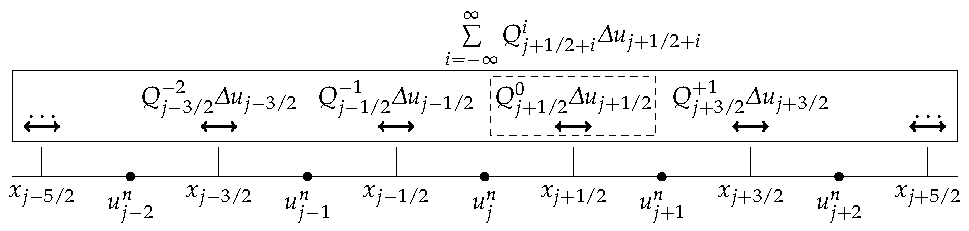
\includegraphics[width=1\textwidth]
	{Figures/Theory/LTSmethod-figure0.eps}}	

	\subfloat[Flux-difference splitting form]
	{\label{fig:LTS-FDS}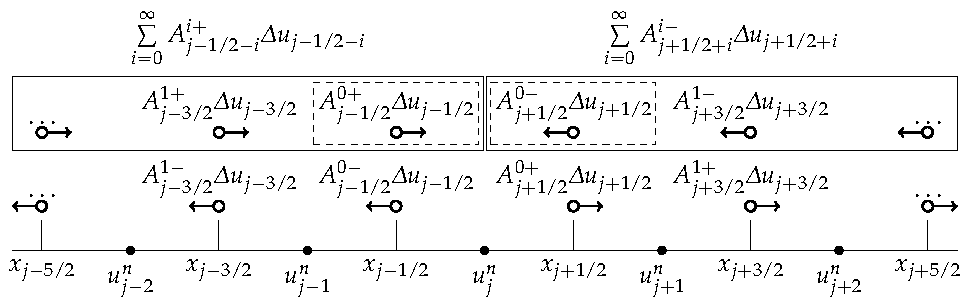
\includegraphics[width=1\textwidth]
	{Figures/Theory/LTSmethod-figure1.eps}}
	
	\captionsetup{justification=centering}
	
	\caption{Updating of $ u_j $: domain of dependence of standard (dashed boxes) and LTS methods (full boxes) in numerical viscosity and flux-difference splitting forms.}
	\label{fig:LTS-methods}
\end{figure} 

The coefficients with the superscript $ 0 $ correspond to the standard methods \eqref{eq:scalar-Q} and \eqref{eq:scalar-A}.

\begin{remark} \label{rem:indexing}
\textup{We note that the absolute cell interface position has a meaning only with respect to a particular cell, for instance $ x_j $ in the examples above. In order to make our definitions of $ Q $ and $ A $ more general, and to simplify the notation, we will suppress the absolute cell interface index. Then, our definition of $ Q $ and $ A $ tells us how the numerical viscosity (or flux-difference splitting) coefficient from an \textit{arbitrary} interface contributes to the numerical flux function (or flux difference) at the interface that is $ |i| $ cells away.
}
\end{remark}

Lindqvist et al.~\cite{lin16} determined the partial viscosity coefficients of the LTS-Roe scheme:
\begin{subequations} \label{eq:scalar-LTS-Roe-NV}
\begin{align}
Q_\text{Roe}^0 & = | \lambda |, \\
Q_\text{Roe}^{\mp i} & = 2 \max \left( 0, \pm \lambda - i \frac{\Delta x}{\Delta t} \right) \quad \text{for} \quad i \; \textgreater \; 0,
\end{align}
\end{subequations}
the LTS-Godunov scheme:
\begin{equation} \label{eq:scalar-LTS-God-NV}
Q_\text{God}^i = \left\{ \begin{array}{lll}
2 \frac{\left( f(u) + iu\frac{\Delta x}{\Delta t} \right)_{j+1} - \mathcal{M}_{j+1/2}\left( f(u) + iu \frac{\Delta x}{\Delta t} \right)}{u_{j+1} - u_j} \quad & \text{for} \quad i < 0, \\[0.5em]
\frac{f_j + f_{j+1} - 2 \mathcal{M}_{j+1/2}(f(u))}{u_{j+1} - u_j}	\quad & \text{for} \quad i=0, \\[0.5em]
2 \frac{\left( f(u) + iu\frac{\Delta x}{\Delta t} \right)_{j} - \mathcal{M}_{j+1/2}\left( f(u) + iu \frac{\Delta x}{\Delta t} \right)}{u_{j+1} - u_j}	\quad & \text{for} \quad i > 0, \end{array} \right.
\end{equation}
and the LTS-Lax-Friedrichs scheme:
\begin{subequations} \label{eq:scalar-LTS-LxF-NV}
\begin{align}
Q_\text{LxF}^0 & = k \frac{\Delta x}{\Delta t}, \\
Q_\text{LxF}^{\mp i} & = \frac{k-i}{k} \left( \pm \lambda + k \frac{\Delta x}{\Delta t} \right) \quad \text{for} \quad i>0.
\end{align}
\end{subequations}
Lindqvist et al.~\cite{lin16} also determined the flux-difference splitting coefficients of the LTS-Roe scheme:
\begin{equation} \label{eq:scalar-LTS-Roe-FDS}
A_\text{Roe}^{i\pm} = \pm \max \left( 0, \min \left( \pm \lambda - i \frac{\Delta x}{\Delta t}, \frac{\Delta x}{\Delta t} \right) \right),
\end{equation}
and the LTS-Godunov scheme:
\begin{subequations} \label{eq:scalar-LTS-God-FDS}
\begin{align}
A_{\text{God},j-1/2-i}^{i+}
& = \frac{1}{\Delta u_{j-1/2-i}} \left( 
\mathcal{M}_{j-1/2-i} \left( f(u) - \left( i+1 \right) u \frac{\Delta x}{\Delta t} \right) \right. \notag \\
& \left. - 
\mathcal{M}_{j-1/2-i} \left( f(u) - iu \frac{\Delta x}{\Delta t} \right) + u_{j-i} \frac{\Delta x}{\Delta t} \right), \\
A_{\text{God},j+1/2+i}^{i-}
& = \frac{1}{\Delta u_{j+1/2+i}} \left( 
\mathcal{M}_{j+1/2+i} \left( f(u) + i u \frac{\Delta x}{\Delta t} \right) \right. \notag \\
& \left. - 
\mathcal{M}_{j+1/2+i} \left( f(u) + \left( i+1 \right)u \frac{\Delta x}{\Delta t} \right) + u_{j+i} \frac{\Delta x}{\Delta t} \right),
\end{align}
\end{subequations}
while Bore~\cite{bor15} determined them for the LTS-Lax-Friedrichs scheme:
\begin{equation} \label{eq:scalar-LTS-LxF-FDS}
A_{\text{LxF}}^{i\pm} = \frac{1}{2 k} \left( \lambda \pm k \frac{\Delta x}{\Delta t} \right).
\end{equation}
We note that for $ k=1 $, \eqref{eq:scalar-LTS-NV} and \eqref{eq:scalar-LTS-FDS} reduce to \eqref{eq:scalar-NV} and \eqref{eq:scalar-FDS}, respectively. Lindqvist et al.~\cite{lin16} also showed that there is a one-to-one mapping between the numerical viscosity and the flux-difference splitting coefficients:
\begin{lemma}[Lindqvist et al.~\cite{lin16}]
For a given local multi-point scheme, there is a one-to-one mapping between the coefficients $ A $ of \eqref{eq:scalar-LTS-FDS} and the coefficients $ Q $ of \eqref{eq:scalar-LTS-NV} as follows:
\begin{subequations} \label{eq:NV-FDS}
\begin{align}
A^{0\pm} & = \frac{1}{2} \left( \lambda \pm Q^0 \mp Q^{\mp 1} \right), \\
A^{i\pm} & = \pm \frac{1}{2} \left( Q^{\mp i} - Q^{\mp (i+1)}\right), \quad i \, \in \, \{1,\dots,k-1\},
\end{align}
\end{subequations}
and:
\begin{equation} \label{eq:FDS-NV}
Q^i = \left\{ \begin{array}{lll}
2 \sum_{p=-i}^{\infty}			A^{p+} \qquad \quad & \text{for} \quad i<0, \\[0.25em]
  \sum_{p=0} ^{\infty} \left( A^{p+} - A^{p-} \right) & \text{for} \quad i=0, \\[0.25em]
-2 \sum_{p=i} ^{\infty} 		A^{p-} \quad & \text{for} \quad i>0. \end{array} \right.
\end{equation}
\end{lemma}

We will denote the methods \eqref{eq:scalar-LTS-Roe-NV}--\eqref{eq:scalar-LTS-LxF-NV} and \eqref{eq:scalar-LTS-Roe-FDS}--\eqref{eq:scalar-LTS-LxF-FDS} as LTS \textit{one-parameter} methods. Namely, even though the numerical flux function \eqref{eq:scalar-LTS-NV} may depend on more than one numerical viscosity coefficient $ Q $, these methods are natural extensions of the standard one-parameter methods.

\subsection{Convergence and entropy stability}
\label{sec:Background:C-ES-scalar-LTS}

\subsubsection*{Convergence}

The Lax-Wendroff theorem from \cref{sec:SCL-FVM-standard-theory} also applies to LTS methods. The conservation form is ensured by writing the LTS methods in the form \eqref{eq:scalar-LTS-NV}, while the consistency of the LTS-Godunov, LTS-Roe and LTS-Lax-Friedrichs schemes can be shown by using modified equation. The first-order accurate LTS method gives a second-order accurate approximation to the equation (see~\cite{lin16}):
\begin{equation} \label{eq:LTS-ME}
u_t + f(u)_x = \frac{1}{2} \frac{\Delta x^2}{\Delta t} \left[ \left( \sum\limits_{i=1-k}^{k-1} \frac{\Delta t}{\Delta x} \bar{Q}^i - c^2 \right) u_x \right]_x.
\end{equation}
By using any $ Q $ from \eqref{eq:scalar-LTS-Roe-NV}--\eqref{eq:scalar-LTS-LxF-NV} in \eqref{eq:LTS-ME}, by keeping $ c=\text{const.} $ and by passing $ \Delta x \rightarrow 0 $ we recover the scalar conservation law \eqref{eq:SCL}.

The notion of TVD stability was generalized for multi-point schemes by Jameson and Lax~\cite{jam86,jam87} (see also Lindqvist et al.~\cite{lin16}):
\begin{lemma}
A multi-point conservative scheme in the form \eqref{eq:scalar-LTS-NV} is unconditionally TVD if and only if:
\begin{subequations} \label{eq:LTS-TVD}
\begin{align}
2 \left( \Delta x / \Delta t \right) - 2 Q_{j+1/2}^0 + Q_{j+1/2}^{-1} + Q_{j+1/2}^1 & \geq 0, \label{eq:LTS-TVD-a} \\
Q_{j+1/2}^0 - 2 Q_{j+1/2}^{\pm 1} + Q_{j+1/2}^{\pm 2} \mp \lambda_{j+1/2} & \geq 0, \label{eq:LTS-TVD-b} \\
Q_{j+1/2}^{\pm i} - 2 Q_{j+1/2}^{\pm (i+1)} + Q_{j+1/2}^{\pm (i+2)} & \geq 0, \quad \forall \, i \geq 1, \quad \forall \, j. \label{eq:LTS-TVD-c}
\end{align}
\end{subequations}
\end{lemma}
LeVeque~\cite{lev84} showed that the LTS-Godunov scheme is TVD, while Lindqvist et al.~\cite{lin16} showed that the LTS-Roe and LTS-Lax-Friedrichs schemes are also TVD. Further, the property that the Roe and Lax-Friedrichs schemes are the least and most diffusive possible TVD schemes also holds in the LTS framework, where the coefficients of the LTS-Roe and the LTS-Lax-Friedrichs schemes are the least and the most diffusive coefficients possible, respectively. 

\subsubsection*{Entropy stability}
\label{sec:LTS-entropy-stability}

Entropy stability of LTS methods is less understood than that of standard methods. In one of the papers on the LTS-Godunov method, LeVeque conjectured that the LTS-Godunov method converges to the entropy solution \textit{provided the correct entropy solution is used for each Riemann problem}~\cite{lev84}. However, rigorous proof turned out to be very difficult to obtain and to this day it remains an open question.

Contributions to this matter have been made by Wang and Warnecke~\cite{wan93a,wan93b} in the nineteen nineties, where they proved that the LTS-Godunov and LTS-Glimm schemes are entropy stable for $ \bar{C} \leq 2 $ if the flux function is monotone, and for an arbitrary Courant number if the initial data is monotone. Later, Wang et al.~\cite{wan04} proved entropy stability of the LTS-Godunov method for any Courant number for some additional types of initial data. An example of monotone, hence entropy stable LTS method is an LTS version of Lax-Friedrichs scheme studied by Tang and Warnecke~\cite{tan04}. In \cref{sec:PP}, we will show that the LTS-Lax-Friedrichs scheme of Lindqvist et al.~\cite{lin16} is entropy stable by showing it is monotone. An interesting result related to this matter is a monotone, entropy stable LTS-Engquist-Osher scheme by Brenier~\cite{bre84}. Therein, author considers averaged multivalued solutions, and the LTS-Engquist-Osher scheme is deduced from the transport-collapse operator.\footnote{Brenier's framework is quite different than the one considered in this thesis, and it remains to be explored how to compare it to the entropy violating LTS-Engquist-Osher scheme we will derive in \cref{cha:LTS-HLL}.}\textsuperscript{,}\footnote{An important point arising here is that LTS extensions of standard methods are not unique. This will be addressed in \cref{cha3:sec:LTS-one-parameter}.}

Since the numerical viscosity coefficients of some LTS methods were given only recently by Lindquist et al.~\cite{lin16}, we are not familiar with analysis of entropy stability along the lines of work by Osher~\cite{osh84} and Tadmor~\cite{tad84} where the numerical viscosity coefficients $ Q $ are compared to the numerical viscosity coefficient of the Godunov scheme. One difficulty that immediately arises is that in LTS methods, the numerical diffusion in the numerical flux function \eqref{eq:scalar-LTS-NV} is not uniquely determined by a single $ Q $. This leads to a possibility that different combinations of $ Q $ may result in the same overall amount of numerical diffusion.

The recent paper by Lindqvist et al.~\cite{lin16} addressed question of entropy stability by studying modified equation, an approach which we will employ in \cref{sec:EV-ME}. In~\cite{lin16}, modified equation and numerical experiments are used to demonstrate that the LTS-Roe is not entropy stable. This is expected, since it is an extension of the standard Roe scheme. Further, it is shown that the LTS-Roe scheme leads to an entropy violation even more often than the standard Roe scheme. This observation has been reported by other authors as well. We will return to this point in \cref{sec:EV-ME} where we will discuss entropy stability of LTS methods in more detail. 

\section{Finite volume methods for systems of conservation laws}
\label{sec:Background:FVM-systems}

We consider systems of equations \eqref{eq:HSCL} and apply the integration procedure which we used in \cref{sec:FVM-scalar} to go from the scalar conservation law \eqref{eq:SCL} to the numerical method in conservation form \eqref{eq:scalar-CF}. This results in conservation form:
\begin{equation} \label{eq:system-CF}
\mathbf{U}_j^{n+1} = \mathbf{U}_j - \frac{\Delta t}{\Delta x} \left( \mathbf{F}_{j+1/2} - \mathbf{F}_{j-1/2} \right),
\end{equation}
with the numerical flux function defined as:
\begin{equation} \label{eq:system-LTS-NV}
\mathbf{F}_{j+1/2} = \frac{1}{2} \left( \mathbf{F}_j + \mathbf{F}_{j+1} \right) - \frac{1}{2} \sum\limits_{i=-\infty}^{\infty} \mathbf{Q}_{j+1/2+i}^i \Delta \mathbf{U}_{j+1/2+i},
\end{equation}
where the partial numerical viscosity coefficients $ \mathbf{Q}_{j+1/2+i} $ are now matrices. The corresponding flux-difference splitting form is:
\begin{equation} \label{eq:system-LTS-FDS}
\mathbf{U}_j^{n+1} = \mathbf{U}_j - \frac{\Delta t}{\Delta x} \sum\limits_{i=0}^{\infty} \left( \mathbf{A}_{j-1/2-i}^{i+} \Delta \mathbf{U}_{j-1/2-i} + \mathbf{A}_{j+1/2+i}^{i-} \Delta \mathbf{U}_{j+1/2+i} \right),
\end{equation}
where the flux-difference splitting coefficients $ \mathbf{A}_{j+1/2\mp i}^{i\pm} $ are now matrices. 

We observe that \eqref{eq:system-LTS-NV} and \eqref{eq:system-LTS-FDS} are simply expressions \eqref{eq:scalar-LTS-NV} and \eqref{eq:scalar-LTS-FDS} generalized to systems of equations, where we note that we immediately used generalized LTS expressions because these naturally contain the expressions for standard methods.

In order to generalize the ideas developed for scalar conservation laws in \cref{sec:FVM-scalar} to systems of conservation laws, we follow the standard approach which consists of linearizing the problem \eqref{eq:HSCL} and then applying the theory developed for the scalar conservation laws to each characteristic field. Consider the Roe scheme~\cite{roe81} where the numerical viscosity matrix is given as:
\begin{equation}
\mathbf{Q}_\text{Roe} = | \hat{\mathbf{A}} |,
\end{equation}
where $ \hat{\mathbf{A}} $ is the Roe matrix~\cite{roe81} satisfying following conditions:
\begin{itemize}
\item $ \hat{\mathbf{A}} $ is diagonalizable with real eigenvalues, i.e. it is hyperbolic;
\item if $ \mathbf{U}_j, \mathbf{U}_{j+1} \rightarrow \mathbf{U} $, then $ \hat{\mathbf{A}} \left( \mathbf{U}_j, \mathbf{U}_{j+1} \right) = \mathbf{A} \left( \mathbf{U} \right) $, i.e. it is consistent with the original conservation law;
\item $ \hat{\mathbf{A}} \left( \mathbf{U}_j, \mathbf{U}_{j+1} \right) \left( \mathbf{U}_{j+1} - \mathbf{U}_j \right) = \mathbf{F}_{j+1} - \mathbf{F}_j $.
\end{itemize}
We then diagonalize the numerical viscosity matrix $ \mathbf{Q}^i $ and the flux-difference splitting matrices $ \mathbf{A}^{i \pm} $ with the eigenvectors of the Roe matrix as:
\begin{subequations}
\begin{align}
\mathbf{Q}_{j+1/2}^i & = \left( \hat{\mathbf{R}} \mathbf{\Omega}^i \hat{\mathbf{R}}^{-1} \right)_{j+1/2}, \label{eq:system-LTS-Q} \\
\mathbf{A}_{j+1/2}^{i\pm} & = \left( \hat{\mathbf{R}} \mathbf{\Lambda}^{i\pm} \hat{\mathbf{R}}^{-1} \right)_{j+1/2}, \label{eq:system-LTS-A}
\end{align}
\end{subequations}
where $ \mathbf{\Omega} $ and $ \mathbf{\Lambda} $ are diagonal matrices of eigenvalues:
\begin{subequations}
\begin{align}
\mathbf{\Omega} & = \text{diag} \left( \omega_1, \dots, \omega_N \right), \\
\mathbf{\Lambda} & = \text{diag} \left( \lambda_1, \dots, \lambda_N \right).
\end{align}
\end{subequations}
Lindqvist et al.~\cite{lin16} determined the eigenvalues for the LTS-Roe scheme in the numerical viscosity form:
\begin{subequations}
\begin{align}
\omega_{\text{Roe}}^0 & = | \lambda |, \\
\omega_{\text{Roe}}^{\mp i} & = 2 \max \left( 0, \pm \lambda - i \frac{\Delta x}{\Delta t} \right) \quad \text{for} \quad i > 0,
\end{align}
\end{subequations}
and the flux-difference splitting form:
\begin{equation}
\lambda_{\text{Roe}}^{i\pm} = \pm \max \left( 0, \min \left( \pm \lambda - i \frac{\Delta x}{\Delta t}, \frac{\Delta x}{\Delta t} \right) \right).
\end{equation}
They also obtained the eigenvalues for the LTS-Lax-Friedrichs scheme in the numerical viscosity form:
\begin{subequations}
\begin{align}
\omega_{\text{LxF}}^0 & = k \frac{\Delta x}{\Delta t}, \\
\omega_{\text{LxF}}^{\mp i} & = \frac{k-i}{k} \left( \pm \lambda + k \frac{\Delta x}{\Delta t} \right) \quad \text{for} \quad i > 0,
\end{align}
\end{subequations}
while Bore~\cite{bor15} provided them for the flux-difference splitting form:
\begin{equation}
\lambda_{\text{LxF}}^{i\pm} = \frac{1}{2k} \left( \lambda \pm k \frac{\Delta x}{\Delta t} \right),
\end{equation}
where we note that the operations above are applied in each characteristic field.

\subsection{Convergence and entropy stability}

Even though the Lax-Wendroff theorem also holds for systems of equations~\cite{lev02}, it is in general not possible to prove convergence of numerical methods for systems of conservation laws. In fact, a proof of convergence for any finite volume method for a general system of hyperbolic conservation laws \textit{remains an outstanding open problem}, see Bressan~\cite{bre11}. Situation is better when it comes to entropy stability, and it is possible to prove entropy stability of certain methods, for instance Godunov method~\cite{lev01}, HLLE method~\cite{ein88} and HLLC method with wave velocity estimates according to Bouchut~\cite{bou04}. If these methods converge, we can be confident that they converge to the entropy solution. 

An important contribution to the questions of convergence and entropy stability is the book by Bouchut~\cite{bou04}, where preservation of invariant domains and existence of entropy inequalities are used as stability criteria. Therein, preservation of invariant domains is used to ensure positivity preservation, while existence of entropy inequalities \textit{ensures the computation of admissible discontinuities, and at the same time it provides a global stability, by the property that a quantity measuring the global size of the data should not increase}, see Bouchut~\cite{bou04}. Our investigations of LTS methods for systems of equations will be based on comparison with standard, more established methods and on using well studied test cases. At best, we will give heuristic arguments and conjecture on properties of the methods.
